\documentclass[12pt]{article}

\usepackage[utf8x]{inputenc}%
\usepackage{graphicx}%
\usepackage{bibentry}%
\usepackage{hyperref}%
\usepackage{import}%
\usepackage{amsmath}%
\usepackage[romanian]{babel}%
\usepackage{color}%
\usepackage{algorithm}%
%\usepackage{algorithmic}%
\usepackage[noend]{algpseudocode}%
\usepackage{xfrac}


\author{Tudor Berariu \\ \emph{tudor.berariu@gmail.com} \\ Laboratorul
  AI-MAS \\ Faculatea de Automatică și Calculatoare}
\title{Inteligență Artificială \\ Tema 1: \textbf{Algoritmul A*}}

\begin{document}

\maketitle

\section{Scopul temei}
\label{sec:scop}

Scopul acestei teme îl reprezintă înțelegerea și implementarea
algoritmului \textbf{A*}. Testarea se va face pe un joc simplu pentru
care se cere și găsirea unei euristici cât mai bune pentru aplicarea
algoritmului \textbf{A*}.

\section{Descrierea jocului}
\label{sec:descriere}

\begin{figure}[h!]
  \centering \def\svgwidth{.5\textwidth}\import{./}{example_a.pdf_tex}
  \caption{Stare posibilă în jocul \emph{Unblock}. Obiectivul este
    acela de a duce blocul roșu în extremitatea dreaptă.}
  \label{fig:1}
\end{figure}

Jocul ales pentru demonstrarea utilității algoritmului \textbf{A*}
este \emph{Unblock} \footnote{
  \url{http://www.quickflashgames.com/games/unblock/}}. Acesta se
desfășoară pe o tablă de dimensiune $height \times width$ pe care se
găsesc $N$ blocuri de dimensiune $length_i, 1 \le i \le N$. Acestea
sunt dispuse fie orizontal, fie vertical, așa cum se poate observa în
Figura~\ref{fig:1}. Fiecare bloc poate glisa pe direcția pe care este
poziționat dacă nu se lovește de alte blocuri și nu depășește
marginile tablei (vezi Figura~/ref{fig:2}).

\begin{figure}[h!]
  \centering \def\svgwidth{.5\textwidth}\import{./}{example_c.pdf_tex}
  \caption{Blocul albastru se poate muta în trei poziții: două linii
    mai sus, o linie mai sus sau o linie mai jos.}
  \label{fig:2}
\end{figure}

Scopul jocului este acela ca prin mutări succesive să se aducă blocul
roșu în extremitatea dreaptă, precum în Figura~\ref{fig:3}.

\begin{figure}[h!]
  \centering \def\svgwidth{.5\textwidth}\import{./}{example_b.pdf_tex}
  \caption{Stare finală posibilă a jocului (blocul roșu a ajuns la
    limita din dreapta)}
  \label{fig:3}
\end{figure}

În cadrul acestei teme se vor genera planuri (secvențe de mișcări)
care să ghideze blocul roșu către marginea din dreapta a tablei.

\section{Cerințe}
\label{sec:tasks}

În fișierul \texttt{unblock.rkt} sunt implementate funcția ce întoarce
lista tuturor stărilor următoare posibile pentru una data
(\texttt{get\_reachable\_states(s)}) și o funcție ce verifică dacă o
stare este finală (\texttt{is\_final?(s)}). De asemenea, sunt
implementate căutările în adâncime și în lățime pe care le puteți
folosi ca punct de plecare pentru rezolvarea primei sarcini.

Cerințele aceste teme sunt următoarele:
\begin{description}
\item[a) \texttt{[0.4 puncte]}] Să se implementeze algoritmul
  \textbf{A*} folosind orice euristică admisibilă. Să se compare
  rezultatele algoritmului cu cele ale căutării în adâncime și lățime
  folosind funcția \texttt{compare\_algorithms}.
\item[b) \texttt{[0.1 puncte]}] Să se găsească o euristică cât mai
  informată, care să reducă semnificativ stările explorate față de
  căutarea în adâncime sau în lățime.
\item[c) \texttt{[0.1 puncte]}] Să se demonstreze admisiblitatea
  euristicilor folosite.
\end{description}

Euristicile folosite, precum și demonstrația de la bonus, trebuie
descrise într-un document care să fie inclus în arhiva temei.

\section{Detalii despre fișierul \texttt{unblock.rkt}}
\label{sec:implementare}

\subsection{Algoritmii de căutare}
\label{sec:algs}

\subsubsection*{Abstractizarea problemei propuse}
\label{sec:abs}

Pentru rezolvarea primei cerințe (implementarea \textbf{A*}) folosiți
funcțiile:
\begin{itemize}
\item \texttt{get-reachable-states(current-state)} - care întoarce
  o listă de perechi \texttt{(next-state . action)} ce conțin stări
  următoare cu acțiunile asociate cu care s-a produs tranziția.
\item \texttt{is-final?(state)} - predicat ce întoarce \texttt{\#t}
  dacă argumentul este o stare finală.
\end{itemize}

și implementați funcția \texttt{a\_star(state)}. Vă puteți inspira din
funcțiile \texttt{dfs(state)} și \texttt{bfs(state)}, deja
implementate.

\subsubsection*{Evaluarea soluțiilor}
\label{sec:eval}

Pentru a compara algoritmii, rulați funcția
\texttt{compare-algorithms} care primește trei argumente
\begin{itemize}
\item lista algoritmilor de comparat (funcții ce primesc o tablă :
  starea inițială) și întorc un plan;
\item lista numelor acestor algoritmi;
\item lista tablelor ce trebuie rezolvate (sunt definite în fișier
  câteva scenarii de joc: \texttt{board1}, \texttt{board2}, ...).
\end{itemize}

De exemplu, expresia de mai jos
\begin{verbatim}
(compare-algorithms
    `(,dfs ,bfs ,a-star)
    `("DFS" "BFS" "A*")
    `(,board1 ,board2 ,board3 ,board4 ,board5 
      ,board6 ,board7 ,board8 ,board9 ,board10))
\end{verbatim}
produce următorul rezultat care sumarizează numărul de stări explorate
de fiecare algoritm (desigur, algoritmul \textbf{A*} nu este încă
implementat, dar cu siguranță veți schimba asta):
\begin{verbatim}
+----------+----------+----------+----------+
|  board   |   DFS    |   BFS    |    A*    |
+----------+----------+----------+----------+
|         1|       861|       867|    GREȘIT|
+----------+----------+----------+----------+
|         2|       374|      1069|    GREȘIT|
+----------+----------+----------+----------+
|         3|        55|        85|    GREȘIT|
+----------+----------+----------+----------+
|         4|      1116|      2231|    GREȘIT|
+----------+----------+----------+----------+
|         5|       812|       848|    GREȘIT|
+----------+----------+----------+----------+
|         6|      1357|       517|    GREȘIT|
+----------+----------+----------+----------+
|         7|       468|       601|    GREȘIT|
+----------+----------+----------+----------+
|         8|       781|       791|    GREȘIT|
+----------+----------+----------+----------+
|         9|      7373|      7935|    GREȘIT|
+----------+----------+----------+----------+
|        10|      5060|      7080|    GREȘIT|
+----------+----------+----------+----------+
\end{verbatim}

\subsubsection*{Testele}

În fișier există câteva scenarii reprezentate:
\begin{itemize}
\item \texttt{board0a}, \texttt{board0b}, \texttt{board0c} - table de
  joc simple pentru testare rapidă.
\item \texttt{board1} - \texttt{board5} - primele cinci niveluri de
  aici: \url{http://www.quickflashgames.com/games/unblock/}
\item \texttt{board6} - \texttt{board10} - primele cinci niveluri din
  setul \emph{expert} de aici:
  \url{http://www.quickflashgames.com/games/unblock-2/}
\item \texttt{board11} - scenariu pentru care DFS și BFS nu reușesc să
  rezolve în timp decent
\end{itemize}

\subsubsection*{Vizualizare} Pentru a vizualiza o singură stare puteți
folosi funcția \texttt{display-board(board)}. De exemplu,
\texttt{display-board(board8)} produce imaginea din
Figura~\ref{fig:5}.

\begin{figure}[h!]
  \centering 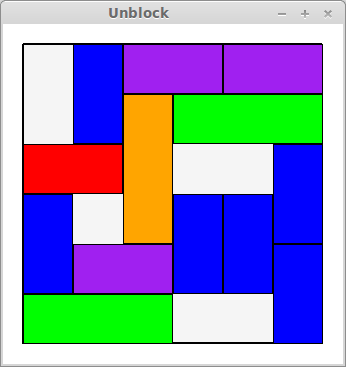
\includegraphics[width=.5\textwidth]{board6.png}
  \caption{Scenariul 6}
  \label{fig:5}
\end{figure}

Pentru a vizualiza un plan aveți la dispoziție funcția
\texttt{display-plan(state0, plan)}, unde \texttt{plan} este o
secvență de mișcări întoarsă de unul dintre algoritmii implementați.

\subsubsection*{Euristici}

Pentru construirea unei euristici cât mai bune, citiți în continuare 
detaliile despre structurile de date ce descriu tabla și blocurile.

\subsection{Structurile de date specifice jocului}
\label{sec:datastructs}

În fișierul \texttt{unblock.rkt} se găsesc definițiile a trei
structuri:
\begin{description}
\item[block] - structură cu trei câmpuri ce reprezintă definiția unui
  bloc:
  \begin{description}
  \item[name] numele asociat blocului;
  \item[orientation] variabilă ce indică dacă un bloc este orientat
    orizontal sau vertical (are valoarea \texttt{HORIZONTAL} sau
    \texttt{VERTICAL};
  \item[length] lungimea blocului.
  \end{description}
\begin{verbatim}
    (struct block (name orientation length))
\end{verbatim}
\item[block-on-board] - structură ce extinde un bloc cu poziția pe
  tablă:
  \begin{description}
  \item[row] linia pe tablă
  \item[column] coloana pe tablă
  \end{description}
\begin{verbatim}
    (struct block-on-board block (row column))
\end{verbatim}
\item[board] - structură ce reprezintă starea tablei la un moment dat:
  \begin{description}
  \item[height] - înălțimea (numărul de linii ale) tablei;
  \item[width] - lățimea (numărul de coloane ale) tablei;
  \item[blocks] - tabelă de dispersie având chei numele blocurilor și
    valori structuri de tip \texttt{block} (descrise mai sus).
  \end{description}
\end{description}
\begin{verbatim}
    (struct board (height width blocks))
\end{verbatim}

\begin{figure}[h!]
  \centering \def\svgwidth{.3\textwidth}\import{./}{exemplu2.pdf_tex}
  \caption{Scenariul \texttt{board0b}.}
  \label{fig:4}
\end{figure}

Exemplu de configurație inițială de joc (corespunzătoare Figurii~\ref{fig:4}):
\begin{verbatim}
(define board0b
  (board 4 4
         (hash "red" (block-on-board "red" HORIZONTAL 2 1 0)
               "blue1" (block-on-board "blue1" VERTICAL 2 0 2)
               "blue2" (block-on-board "blue2" VERTICAL 2 1 3)
              )))
\end{verbatim}
Un plan generat prin căutare în adâncime este:
\begin{verbatim}
> (dfs board0b)
'(("blue2" -1 0) ("blue2" 2 0) ("blue1" 1 0) ("blue2" -1 0)
  ("blue2" -1 0) ("blue1" 1 0) ("red" 0 1) ("blue2" 1 0)
  ("red" 0 -1) ("blue2" 1 0) ("red" 0 1) ("red" 0 1))
\end{verbatim}

Funcțiile \texttt{print-plan(plan)} și \texttt{display-plan(board,
  plan)} ajută la descifrarea planului:
\begin{verbatim}
> (print-plan (dfs board0b))
  1. Move block 'blue2' -1 rows, 0 columns.
  2. Move block 'blue2' 2 rows, 0 columns.
  3. Move block 'blue1' 1 rows, 0 columns.
  4. Move block 'blue2' -1 rows, 0 columns.
  5. Move block 'blue2' -1 rows, 0 columns.
  6. Move block 'blue1' 1 rows, 0 columns.
  7. Move block 'red' 0 rows, 1 columns.
  8. Move block 'blue2' 1 rows, 0 columns.
  9. Move block 'red' 0 rows, -1 columns.
  10. Move block 'blue2' 1 rows, 0 columns.
  11. Move block 'red' 0 rows, 1 columns.
  12. Move block 'red' 0 rows, 1 columns.
\end{verbatim}

Funcția care întoarce toate stările în care se poate ajunge dintr-o
stare curentă este \texttt{get-reachable-states(s)}. De exemplu,
pentru starea inițială \texttt{board0b}:

\begin{verbatim}
> (get-reachable-states board0b)
(((board 4 4
         (hash "red" (block-on-board "red" 2049 2 1 0)
               "blue2" (block-on-board "blue2" 2048 2 0 3)
               "blue1" (block-on-board "blue1" 2048 2 0 2)))
   . ("blue2" -1 0))
 ((board 4 4
         (hash "red" (block-on-board "red" 2049 2 1 0)
    "blue2" (block-on-board "blue2" 2048 2 2 3)
    "blue1" (block-on-board "blue1" 2048 2 0 2)))
   . ("blue2" 1 0))
 ((board 4 4
         (hash "red" (block-on-board "red" 2049 2 1 0)
               "blue2" (block-on-board "blue2" 2048 2 1 3)
               "blue1" (block-on-board "blue1" 2048 2 1 2)))
   . ("blue1" 1 0))
 ((board 4 4
         (hash "red" (block-on-board "red" 2049 2 1 0)
               "blue2" (block-on-board "blue2" 2048 2 1 3)
               "blue1" (block-on-board "blue1" 2048 2 2 2)))
  . ("blue1" 2 0)))
\end{verbatim}

Rezultatul conține patru perechi $(stare . acțiune)$ unde $stare$
reprezintă o nouă configurație a blocurilor, iar $acțiune$ este o
listă compusă din numele blocului mutat, numărul de linii și numărul
de coloane pe care s-a deplasat.

\textbf{Succes!}

\end{document}
